% assignment_3.tex - Assignment 3 for Machine Learning class (Spring 2015)
% Chanmann Lim - March 2015

\documentclass[a4paper]{article}

\usepackage[margin=1 in]{geometry}
\usepackage{amsmath}
\usepackage{listings}
\usepackage{graphicx}
\usepackage[T1]{fontenc}
\usepackage{float}
\usepackage{multirow}
\usepackage{rotating}

\everymath{\displaystyle}

\begin{document}
\setcounter{page}{3}
% \thispagestyle{empty}
% \pagestyle{empty}

% Part I
\subsection*{3. Part I}

% a
\paragraph{a.} $\mu$ and $\Sigma$ from the first 10 data samples: \\
\begin{align*}
	\mu = \begin{bmatrix}
		0.8190 & -0.6271
	\end{bmatrix}^{T}, \quad
	\Sigma = \begin{bmatrix}
		 0.7461  &  -0.1474 \\
		-0.1474  &   1.6047
	\end{bmatrix}
\end{align*}

% b
\paragraph{b.} $\mu$ and $\Sigma$ from the first 100 data samples: \\
\begin{align*}
	\mu = \begin{bmatrix}
		0.9977 & -0.9725
	\end{bmatrix}^{T}, \quad
	\Sigma = \begin{bmatrix}
		2.2580  &  1.0856 \\
		1.0856  &  2.1439
	\end{bmatrix}
\end{align*}

% c
\paragraph{c.} $\mu$ and $\Sigma$ from the first 1000 data samples: \\
\begin{align*}
	\mu = \begin{bmatrix}
		1.0222 & -0.9629
	\end{bmatrix}^{T}, \quad
	\Sigma = \begin{bmatrix}
		2.2118  &  1.1878 \\
		1.1878  &  2.0332
	\end{bmatrix}
\end{align*}

% d
\paragraph{c.} $\mu$ and $\Sigma$ from the first 10000 data samples: \\
\begin{align*}
	\mu = \begin{bmatrix}
		0.9947 & -1.0027
	\end{bmatrix}^{T}, \quad
	\Sigma = \begin{bmatrix}
		1.9978  &  0.9643 \\
		0.9643  &  1.9237
	\end{bmatrix}
\end{align*}

% e
\paragraph{e.} Parameter estimation errors \\

Measure 1:
	\begin{tabular}{l *{4}{c}}
			case      &   a    &   b    &   c    &   d    \\ \hline
		$\varepsilon$ & 1.7935 & 0.3088 & 0.2883 & 0.0845
	\end{tabular} \\
\vspace{2em}
 
Measure 2:
	\begin{tabular}{l *{4}{c}}
				case            &   a    &   b    &   c    &   d    \\ \hline
		$\varepsilon _{\mu}$    & 0.2931 & 0.0195 & 0.0306 & 0.0042 \\ 
		$\varepsilon _{\Sigma}$ & 1.0075 & 0.1776 & 0.1646 & 0.0487 
	\end{tabular} \\
\vspace{2em}

In \emph{Measure 1}, the estimation error declines as more data are obtained, however it is not all the cases in \emph{Measure 2} as we observe the estimation error in mean $\varepsilon _{\mu}$ and the estimation error in covariance $\varepsilon _{\Sigma}$ differently. When 100 samples are used to learn parameter $\boldsymbol{\theta}$, the error in mean increase compared to when only 10 samples are being fed into the MLE estimator and this phenomenon can be explained by the sensitivity of the mean measure to outlier in the samples data.

% f
\paragraph{e.} Plot of first 100 data samples and 2D contours of estimated Gaussian pdf \\
\begin{figure}[H]
  \centering
    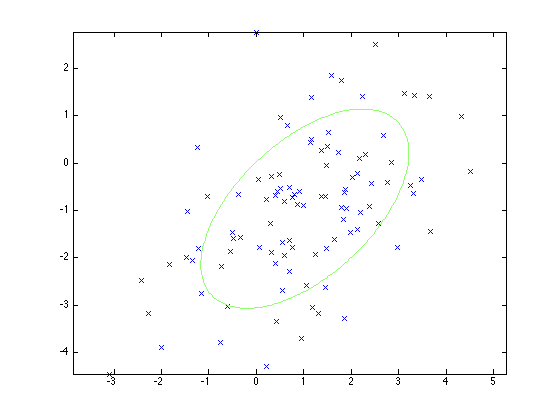
\includegraphics[scale=.47]{images/3_f_I.png}
  \caption{100 data samples and estimated Gaussian pdf 2D contours}
\end{figure}

% Part II
\subsection*{Part II}

% a
\paragraph{a.} $\mu$ and $\Sigma$ from the first 10 data samples: \\
\begin{align*}
	\mu = \begin{bmatrix}
		1.8829 & -1.8135
	\end{bmatrix}^{T}, \quad
	\Sigma = \begin{bmatrix}
		 5.6385  & -5.3104 \\
		-5.3104  &  5.3521
	\end{bmatrix}
\end{align*}

% b
\paragraph{b.} $\mu$ and $\Sigma$ from the first 100 data samples: \\
\begin{align*}
	\mu = \begin{bmatrix}
		1.1741 & -1.2216
	\end{bmatrix}^{T}, \quad
	\Sigma = \begin{bmatrix}
		 2.6753  & -2.5961 \\
		-2.5961  &  2.6913
	\end{bmatrix}
\end{align*}

% c
\paragraph{c.} $\mu$ and $\Sigma$ from the first 1000 data samples: \\
\begin{align*}
	\mu = \begin{bmatrix}
		0.9539 & -0.9530
	\end{bmatrix}^{T}, \quad
	\Sigma = \begin{bmatrix}
		 1.9939  & -1.9344 \\
		-1.9344  &  2.0528
	\end{bmatrix}
\end{align*}

% d
\paragraph{c.} $\mu$ and $\Sigma$ from the first 10000 data samples: \\
\begin{align*}
	\mu = \begin{bmatrix}
		1.0023 & -1.0031
	\end{bmatrix}^{T}, \quad
	\Sigma = \begin{bmatrix}
		 1.9659  & -1.8639 \\
		-1.8639  &  1.9582
	\end{bmatrix}
\end{align*}

% e
\paragraph{e.} Parameter estimation errors \\

Measure 1:
	\begin{tabular}{l *{4}{c}}
			case      &   a    &   b    &   c    &   d    \\ \hline
		$\varepsilon$ & 6.1275 & 1.2239 & 0.0914 & 0.0651
	\end{tabular} \\
\vspace{2em}
 
Measure 2: 
	\begin{tabular}{l *{4}{c}}
				case            &   a    &   b    &   c    &   d    \\ \hline
		$\varepsilon _{\mu}$    & 0.8489 & 0.1993 & 0.0466 & 0.0028 \\ 
		$\varepsilon _{\Sigma}$ & 3.4692 & 0.6876 & 0.0366 & 0.0375 
	\end{tabular} \\
\vspace{2em}

In both \emph{Measure 1} and \emph{Measure 2} we notice that parameter estimation errors decrease as the number of data samples increase. Maximum likelihood estimation assumes that the parameter $\boldsymbol{\theta}$ is fixed then seeks to find the parameter value that maximizes the probability of the training data being observed.

% f
\paragraph{e.} Plot of first 100 data samples and 2D contours of estimated Gaussian pdf \\
\begin{figure}[H]
  \centering
    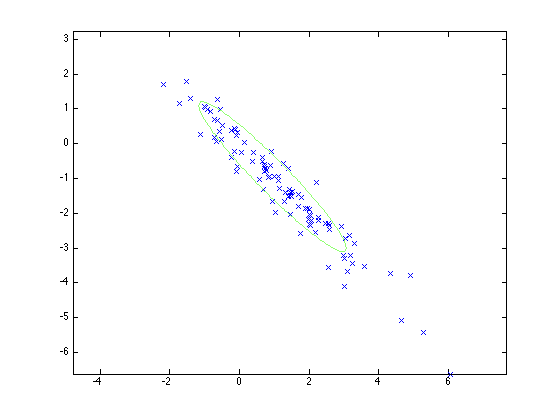
\includegraphics[scale=.47]{images/3_f_II.png}
  \caption{100 data samples and estimated Gaussian pdf 2D contours}
\end{figure}

% Prob. 4
\subsection*{4.}

% a
\paragraph{a.} ~\\
\begin{align*}
	\mu_{MLE} = \begin{bmatrix}
		4.2897 \\
    	3.1275 \\
    	2.9466 \\
    	2.6994 \\
    	2.5360 \\
    	2.3195 \\
    	2.1012 \\
    	2.1773 \\
    	2.1529 \\
    	1.9803 \\
    	1.9825 \\
    	2.0185 \\
    	1.9584 \\
    	1.9170 \\
    	1.9686 \\
    	1.9283 \\
    	1.9663 \\
    	1.9756 \\
    	1.9851 \\
    	2.0310
	\end{bmatrix}, \quad
	\mu_{MAP} = \begin{bmatrix}
		2.6179 \\
    	2.5975 \\
    	2.6148 \\
    	2.5178 \\
    	2.4326 \\
    	2.2876 \\
    	2.1245 \\
    	2.1821 \\
   		2.1618 \\
    	2.0185 \\
    	2.0173 \\
    	2.0454 \\
    	1.9917 \\
    	1.9535 \\
    	1.9966 \\
    	1.9593 \\
    	1.9915 \\
    	1.9986 \\
    	2.0061 \\
    	2.0467
	\end{bmatrix}
\end{align*}

% b
\paragraph{b.} Plot of the error curves of MLE and MAP:\\
\begin{figure}[H]
  \centering
    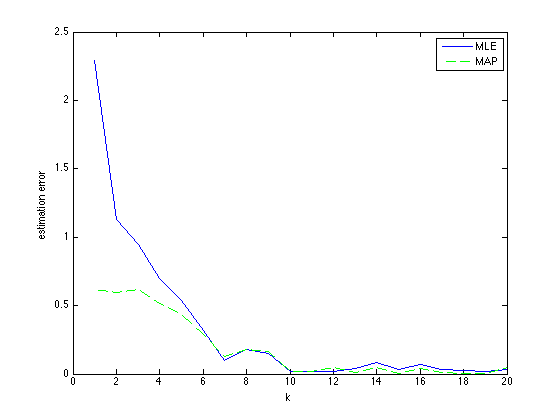
\includegraphics[scale=.47]{images/4_esti_error.png}
  \caption{Error curves when $\mu_{true} = 2$}
\end{figure}

MLE performs poorly compared to MAP when there is less training data available and sometimes the error is too high to to be acceptable and should not be used however when samples data is abundant MLE estimation is almost as good as MAP method which requires much more computational power to evaluate.

% c
\paragraph{c.} Plot of the $\mu \sim N(\mu_{N}, \sigma^{2}_{N})$ for k=1, 10 and 20:\\
\begin{figure}[H]
  \centering
    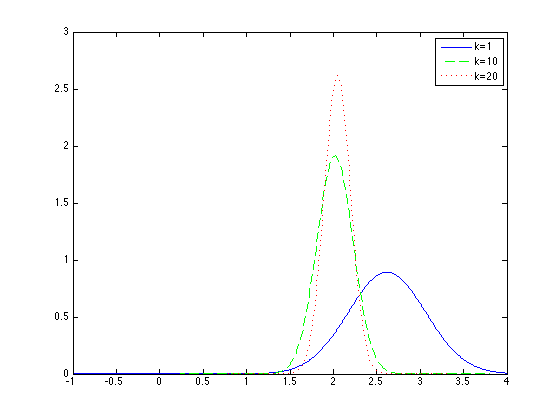
\includegraphics[scale=.47]{images/4_posterior_pdf.png}
  \caption{$\mu \sim N(\mu_{N}, \sigma^{2}_{N}), \quad k=\{1, 10, 20\}$}
\end{figure}

All posterior probability density functions of $\mu \sim N(\mu_{N}, \sigma^{2}_{N})$ when k=1, 10 and 20 have different mean and variance and by observing the variance of each PDF we notice that the PDF of $\mu$ when k=1 has the widest spread in $x$ direction than other densities which indicates the poor quality of its estimated mean and in the case of k=20 the variance measure become smaller than the other two curves hence the estimated mean when k=20 is more accurate than when k=1 and k=10. In treating the parameter $\boldsymbol{\theta}$ as a random variable in MAP estimation, the estimated $\mu$ can be improved significantly as new training data is obtained.

% Prob. 4
\subsection*{4. Experiment 1}

% b
\paragraph{b.} MLE estimates of the mean and diagonal covariance matrix: \\
\begin{align*}
	\mu_{(x|\omega=\text{Iris-setosa})} = \begin{bmatrix}
		5.0967 \\
    	3.4833 \\
    	1.4667 \\
    	0.2367
	\end{bmatrix}, \quad
	\Sigma_{(x|\omega=\text{Iris-setosa})} = \begin{bmatrix}
	0.1310  &       0  &       0  &       0\\
         0  &  0.1367  &       0  &       0\\
         0  &       0  &  0.0349  &       0\\
         0  &       0  &       0  &  0.0110
	\end{bmatrix}
\end{align*}
\begin{align*}
	\mu_{(x|\omega=\text{Iris-versicolor})} = \begin{bmatrix}
		5.9800\\
	    2.7500\\
    	4.3000\\
	    1.3400
	\end{bmatrix}, \quad
	\Sigma_{(x|\omega=\text{Iris-versicolor})} = \begin{bmatrix}
	0.1936  &       0  &       0  &       0\\
         0  &  0.1058  &       0  &       0\\
         0  &       0  &  0.1920  &       0\\
         0  &       0  &       0  &  0.0471
	\end{bmatrix}
\end{align*}
\begin{align*}
	\mu_{(x|\omega=\text{Iris-virginica})} = \begin{bmatrix}
		6.6400\\
	    2.9667\\
	    5.5533\\
	    1.9733
	\end{bmatrix}, \quad
	\Sigma_{(x|\omega=\text{Iris-virginica})} = \begin{bmatrix}
	0.4131  &       0  &       0  &       0\\
         0  &  0.1129  &       0  &       0\\
         0  &       0  &  0.3292  &       0\\
         0  &       0  &       0  &  0.0700
	\end{bmatrix}
\end{align*}

% c
\paragraph{c.} Confusion table:\\

\begin{tabular}{|r| *{3}{c|}}
	\hline
	\multirow{2}{*}{True class} 
				& \multicolumn{3}{ c| }{Classified class} \\ \cline{2-4}
				& Setosa & Versicolor & Virginica\\ \hline
	Setosa 		& 20 &  0 &  0\\ \hline
	Versicolor	&  0 & 19 &  1\\ \hline
	Virginica	&  0 &  1 & 19\\ \hline
	
\end{tabular}

% Experiment 2
\subsection*{Experiment 2}

% b
\paragraph{b.} MLE estimates of the mean and full covariance matrix: \\
\begin{align*}
	\mu_{(x|\omega=\text{Iris-setosa})} = \begin{bmatrix}
		5.0967\\
	    3.4833\\
	    1.4667\\
	    0.2367
	\end{bmatrix}, \quad
	\Sigma_{(x|\omega=\text{Iris-setosa})} = \begin{bmatrix}
	0.1310  &  0.0973  &  0.0102  &  0.0141\\
    0.0973  &  0.1367  & -0.0032  &  0.0133\\
    0.0102  & -0.0032  &  0.0349  &  0.0046\\
    0.0141  &  0.0133  &  0.0046  &  0.0110
	\end{bmatrix}
\end{align*}
\begin{align*}
	\mu_{(x|\omega=\text{Iris-versicolor})} = \begin{bmatrix}
		5.9800\\
	    2.7500\\
    	4.3000\\
	    1.3400
	\end{bmatrix}, \quad
	\Sigma_{(x|\omega=\text{Iris-versicolor})} = \begin{bmatrix}
	0.1936  &  0.0510  &  0.1247  &  0.0428\\
    0.0510  &  0.1058  &  0.0633  &  0.0450\\
    0.1247  &  0.0633  &  0.1920  &  0.0757\\
    0.0428  &  0.0450  &  0.0757  &  0.0471
	\end{bmatrix}
\end{align*}
\begin{align*}
	\mu_{(x|\omega=\text{Iris-virginica})} = \begin{bmatrix}
		6.6400\\
	    2.9667\\
	    5.5533\\
	    1.9733
	\end{bmatrix}, \quad
	\Sigma_{(x|\omega=\text{Iris-virginica})} = \begin{bmatrix}
	0.4131  &  0.1013  &  0.3309  &  0.0417\\
    0.1013  &  0.1129  &  0.0718  &  0.0341\\
    0.3309  &  0.0718  &  0.3292  &  0.0484\\
    0.0417  &  0.0341  &  0.0484  &  0.0700
	\end{bmatrix}
\end{align*}

% c
\paragraph{c.} Confusion table:\\

\begin{tabular}{|r| *{3}{c|}}
	\hline
	\multirow{2}{*}{True class} 
				& \multicolumn{3}{ c| }{Classified class} \\ \cline{2-4}
				& Setosa & Versicolor & Virginica\\ \hline
	Setosa 		& 20 &  0 &  0\\ \hline
	Versicolor	&  0 & 20 &  0\\ \hline
	Virginica	&  0 &  0 & 20\\ \hline
	
\end{tabular}


\newpage
\subsection*{Appendix:}
\lstinputlisting[language=Matlab, title=\lstname, basicstyle=\footnotesize]{assignment_3.m}
\lstinputlisting[language=Matlab, title=\lstname, basicstyle=\footnotesize]{problem_3_report.m}
\lstinputlisting[language=Matlab, title=\lstname, basicstyle=\footnotesize]{mle.m}
\lstinputlisting[language=Matlab, title=\lstname, basicstyle=\footnotesize]{theta.m}
\lstinputlisting[language=Matlab, title=\lstname, basicstyle=\footnotesize]{error_measure_1.m}
\lstinputlisting[language=Matlab, title=\lstname, basicstyle=\footnotesize]{error_measure_2.m}
\lstinputlisting[language=Matlab, title=\lstname, basicstyle=\footnotesize]{problem_4_report.m}
\lstinputlisting[language=Matlab, title=\lstname, basicstyle=\footnotesize]{map.m}
\lstinputlisting[language=Matlab, title=\lstname, basicstyle=\footnotesize]{normal1.m}
\lstinputlisting[language=Matlab, title=\lstname, basicstyle=\footnotesize]{problem_5_report.m}
\lstinputlisting[language=Matlab, title=\lstname, basicstyle=\footnotesize]{classify.m}
































\end{document}